\chapter{Code}

\section{Arduino Enviroment}

\subsection{Arduino Coding Environment}
To write code for Arduino devices, you need an IDE\footnote{Integrated development environment}. An IDE normally consists of a source code editor, build automation tools, and a debugger.  

The most popular IDE is Arduino IDE, which is very beginner friendly, but it has it's weaknesses when it comes to writing code, for instance the lacking of $intelliSense$\footnote{IntelliSense is a code-completion aid that includes a number of features: List Members, Parameter Info, Quick Info, and Complete Word.}. This is not an issue when making a small project, like making a LED blink. But when it comes to bigger projects, which have many components and 3rd party libraries, coding becomes very hard without intelliSense. Another disadvantage with Arduino IDE, is when working with many files. The more files the project has the more complicated it becomes to locate them, since it is all set up like a large document instead of small subsections. A small example of this \ref{fig:example}

\newpage

\begin{figure}[!h]
    \centering
    \subfloat[Arduino IDE]{{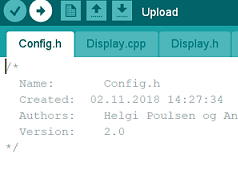
\includegraphics[width=5cm]{fig/arduinofiles} }}%
    \qquad
    \subfloat[Visual Studio 2017]{{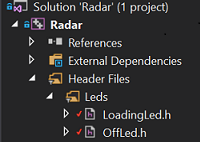
\includegraphics[width=5cm]{fig/vsfiles} }}%
    \caption{Difference in file structure}%
    \label{fig:example}%
\end{figure} 
 

For these reasons and others, Visual Studio was used to create this project.

\subsection{Arduino code}
The Arduino language is merely a set of $C/C++$ functions that can be called from your code. All standard $C$ and $C++$ constructs supported by $avr-g++$ should work in Arduino.\footnote{\url{https://www.arduino.cc/en/Main/FAQ}}

Arduino uses sketches. A sketch is the name that Arduino uses for a program. It's the unit of code that is uploaded to and run on an Arduino board.

Every project must have one main sketch file, which must be an $.INO$ file. This is the file containing the $setup()$ and $loop()$ functions. The $setup()$ runs only once, when the Arduino is powered up. After $setup()$, the $loop()$ function runs  over and over. This means that when $\}$ is reached, it starts from the top again.

$.CPP$ and $.H$ files can also be used and is recommended, since it gives you more control and overview.

\newpage

\section{Libraries}
Libraries are files written in C or C++, which provide your sketches with extra functionality. More information about them can be found at \url{https://www.arduino.cc/en/Main/Libraries}, where even a template is provided so that the user can write his own library.

In this project we used a few libraries:
\begin{multicols}{2}
\begin{itemize}
	\item Servo \textit{Servo}
	\item LiquidCrystal\_I2C \textit{Display}
	\item NewPing \textit{Ultrasonic}	
	\item Wire \textit{Display}	
\end{itemize}
\end{multicols}

\section{Radar.ino}
This is the main file in the project. Here we have included all the header files and created objects that are needed, like the $servo$ and $lcd$ objects that come from the $servo$ and $LiquidCrystal\_I2C$ libraries.

\subsection{void setup()}
\lstinputlisting[language=c++,firstline=33, lastline=51]{Backmatter/Code/Radar.ino}

\subsubsection{Serial.begin(9600)}
Sets the data rate in $bits per second (baud)$ for serial data transmission. For communicating with the computer. The rate set is $9600$.
\subsubsection{Serial.println()}
The serial.println() functions are used for printing the data to the serial port. In this case it is used to get the data into a $Excel$ spreadsheet via a software called $PLX-DAQ$\footnote{PLX-DAQ is a Parallax microcontroller data acquisition add-on tool for Microsoft Excel} for the tests to measure the accuracy of the ultrasonic sensor. More information about $PLX-DAQ$ can be found on \href{https://www.parallax.com/downloads/plx-daq}{PLX-DAQ}  

\subsubsection{Servo}
We initialize the servo here by attaching it to a pin and setting it to position $0$.

\subsubsection{load.blink()}
This is just making the yellow led blink fast multiple times. This just gives the user the sensation that everything is starting up.

\subsubsection{lcd}
here we initialize the lcd display and turn it on. 
$display.intro(lcd)$ is the function that shows the intro screen.

\subsection{void loop()} \label{voidloop}
\lstinputlisting[language=c++,firstline=53, lastline=57]{Backmatter/Code/Radar.ino}

Here is where the magic happens. In our $loop()$, we only have one function, that controls everything.

$run(servo, lcd)$ takes two arguments, the servo object and the lcd object. 

\section{Classes}
We have created a class for each component(sensor,motor,led), since the main purpose of C++ programming is to add object orientation to the C programming language. This gives us much more flexibility with the project and makes it much easier to expand. Each class is also in its own header file. Our classes are:
\begin{itemize}
  \item UltraSonicClass
  \item TemperatureClass
  \item ServoMotorClass
  \item SerialPrintClass
  \item PowerOnOffClass
  \item DisplayClass
  \item LedClass
  \begin{itemize}
     \item LoadingLedClass
     \item OnLedClass
     \item OffLedClass
   \end{itemize}
  \item RGBLedClass
\end{itemize}

We use hierarchical inheritance for the led classes. We wanted to add a factory method design pattern\footnote{\url{https://www.tutorialspoint.com/design_pattern/factory_pattern.htm}} to the led classes, but we encountered some strange object problems.  

\section{Config.h}
The config header file contains the constants for the digital and analog pins. Here we use namespace\footnote{A namespace is a declarative region that provides a scope to the identifiers (names of the types, function, variables etc.) inside it.}

\section{Functions}
This project contains lots of classes and functions. Here we will take a closer look at some of the more complicated and important ones.

\subsection{void run(Servo s, LiquidCrystal\_I2C lcd)\ref{appendix:PowerOnOff}}
As mentioned in \ref{voidloop}, this is the main function. 

$void run(Servo s, LiquidCrystal\_I2C lcd)$ is the button. If turned on, turn the servo, measure  temperature, measure distance and so on. If off, stop everything, turn the the red led on and display the into on the display.

Since the code is heavily commented, to make it as easy to understand as possible, the need to explain each line is not necessary. 

To get the button to work as intended was more complicated that it seemed. 
\newpage

The basic principle of it\ref{fig:btnDiagram}:
\begin{figure}
  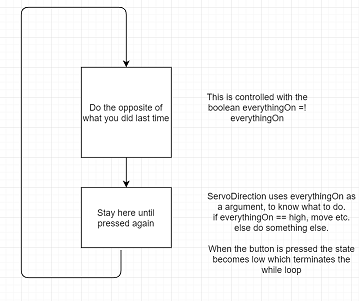
\includegraphics[width=\linewidth]{fig/buttonDiagram}
  \caption{Button diagram}
  \label{fig:btnDiagram}
\end{figure}

\subsection{void servoDirection(Servo s, int state, LiquidCrystal\_I2C lcd)\ref{appendix:PowerOnOff}}
In $void servoDirection(Servo s, int state, LiquidCrystal\_I2C lcd)$.
we check if the state is $HIGH$, then for every 10 counter degrees, we set the temperature and speed of sound. We do this since the temperature module is not stable enough. Then we set the distance in $centimeters$ and then showing the distance with the rgb module and print the important information on the display.

We use a $if$ statement with the argument $up$, that is a boolean, to decide which way the servo goes. If up is true then go from $min$ to $max$, else go from $max$ to $min$. 

The $counter$ is the servo position. So when $counter$ reaches $max$, we set up $= false$.

the string $leftRight$ and integer $test$ are only used for $serialPrint$\ref{appendix:SerialPrint}.

$sm.rotate$\ref{appendix:ServoMotor} is the function that rotates the servo. It takes $servo$ and $counter$ as arguments.

\subsection{void setSpeedOfSound(int temperature)\ref{appendix:UltraSonic}}
To set the speed of sound with temperature, we need to use the speed of sound formula:
\begin{equation}
c = 331.3 \times \sqrt{\frac{\vartheta + 273.15}{273.15}} = 331.3 \times \sqrt{1 + \frac{\vartheta}{273.15}}
\end{equation}
A simplified formula can be used for $\ang{+35} C to \ang{-35} C$

Speed of sound in air in m/s:
\begin{equation}
c=331.3 + 0.6 \times \vartheta
\end{equation}
To make our calculations light weight as possible, we used the the simplified formula.

\subsection{void setDistance(float speedOfSound)\ref{appendix:UltraSonic}}
We found a very good library, $NewPing$, that can measure the distance for the ultrasonic sensor. We decided not to use it since it doesn't take speed of sound as argument and found it better for the project to write the code ourselves. 

We show how to use it in the inline comments if the reader wants to use it instead of our code.

First we set the trigger pin to $LOW$ and make a $4$ microseconds delay to ensure a clean $HIGH$ pulse, then the sensor is triggered by a $HIGH$ pulse of $10$ microseconds.

$duration$ is the time in microseconds from the sending of the ping to the reception of its echo off of an object.

Then we convert the time into $cm$ 
\begin{equation}
distance = \frac{duration \times \frac{speedOfSound}{1000}}{2} 
\end{equation}

\subsection{void setTemperature()\ref{appendix:Temperature}}
To turn the 10-bit analog reading into a temperature:

Formula that converts the number $0/1023$ from Analog ADC input into $0-5000mV(=5V)$:

First we read the analog pin, then:
\begin{equation}
voltage = reading \times 5.0
\end{equation}
then:
\begin{equation}
voltage = \frac{voltage}{1024}
\end{equation}

Convert to Celsius:
\begin{equation}
temperatureCelsius = (voltage - 0.5) \times 100
\end{equation}

